The \mf Streamflow Routing (SFR) Package simulates the interactions between surface-water features and groundwater systems. By default, the SFR Package solves a steady, uniform flow equation for each reach under the assumption that flow adjusts instantaneously within each time step. This chapter describes an optional kinematic wave routing formulation for the SFR Package that accounts for transient storage within stream reaches. The approach is based on the methods described in \cite{McArthur1993} and is equivalent to the ``TRANSROUTE'' option in the SFR Package available in \mfn \citep{modflownwt} and first described in \citet{markstrom2008gsflow}. Accurate representation of flood-wave timing requires that the model time step be comparable to the kinematic-wave travel time through a reach; guidance for selecting the time step is provided in the Practical Guidance section.

\subsection{Kinematic Wave Approximation}

The complete one-dimensional Saint-Venant equations for open-channel flow comprise the continuity equation and the momentum equation. The momentum equation includes terms representing local acceleration, advective acceleration, pressure gradient, gravity, and friction. The kinematic wave approximation retains only the gravity and friction terms in the momentum equation, which is equivalent to assuming that the energy grade line is parallel to the channel bed slope. Under this approximation, the discharge $Q$ ($L^3 T^{-1}$) is uniquely determined by the depth of flow and the channel geometry, and the governing equation reduces to the continuity equation alone \citep{LighthillWhitham1955, PonceSimons1977, PonceLiSimons1978}

\begin{equation}
	\label{eqn:sfr-continuity}
	\frac{\partial Q}{\partial x} + \frac{\partial A}{\partial t} = q_L ,
\end{equation}

\noindent where $Q$ is the volumetric discharge ($L^3 T^{-1}$), $A$ is the cross-sectional area of flow ($L^2$), $x$ is the longitudinal distance along the channel ($L$), $t$ is time ($T$), and $q_L$ is the lateral inflow rate per unit channel length ($L^2 T^{-1}$). The kinematic wave approximation is applicable when the Froude number is less than about 2 and the channel slope is sufficiently steep relative to the backwater effect \citep{McArthur1993, WoolhiserLiggett1967, PonceLiSimons1978, Ponce1991}.

\subsection{Discharge-Depth Relationship}

The discharge in a reach is calculated using Manning's equation \citep{Manning1891}

\begin{equation}
	\label{eqn:sfr-manning}
	Q = \frac{\alpha}{n} A R^{2/3} S_0^{1/2} ,
\end{equation}

\noindent where $\alpha$ is a unit conversion factor ($\alpha = 1$ for SI units; $\alpha = 1.486$ for U.S.~customary units), $n$ is Manning's roughness coefficient ($T L^{-1/3}$), $R$ is the hydraulic radius ($L$) defined as $R = A / P_w$ where $P_w$ is the wetted perimeter ($L$), and $S_0$ is the channel bed slope (dimensionless). Equation~\ref{eqn:sfr-manning} establishes a nonlinear, monotonically increasing relationship between $Q$ and $A$ (or equivalently, between $Q$ and flow depth $d$) for a given channel geometry. This functional relationship is used to determine the depth corresponding to a computed discharge and to evaluate the wet cross-sectional area \citep{chaudhry2008}.

\subsection{Wave Celerity and Courant Number}

The kinematic wave celerity $c$ ($L T^{-1}$) is the speed at which a small perturbation in discharge propagates downstream. It is defined as the derivative of discharge with respect to cross-sectional area

\begin{equation}
	\label{eqn:sfr-celerity}
	c = \frac{dQ}{dA} .
\end{equation}

\noindent In practice, the celerity is evaluated numerically by finite difference as

\begin{equation}
	\label{eqn:sfr-celerity-num}
	c \approx \frac{\delta}{A(Q + \delta) - A(Q)} ,
\end{equation}

\noindent where $\delta$ is a small perturbation in discharge and $A(Q)$ is the cross-sectional area corresponding to discharge $Q$, obtained by inverting Manning's equation (eq.~\ref{eqn:sfr-manning}). For a Manning's-equation-based channel, the kinematic wave celerity is approximately $5/3$ times the mean flow velocity at low depths and may be several times the mean velocity in wide channels \citep{LighthillWhitham1955, chaudhry2008}.

The Courant number $C_r$ (dimensionless) relates the wave celerity to the computational cell size

\begin{equation}
	\label{eqn:sfr-courant}
	C_r = \frac{c \, \Delta t}{\Delta x} ,
\end{equation}

\noindent where $\Delta t$ is the time step length ($T$) and $\Delta x$ is the reach length ($L$). The Courant number governs the temporal weighting used in the finite-difference approximation of equation~\ref{eqn:sfr-continuity}.

\subsection{Finite-Difference Discretization}

A four-point implicit finite-difference scheme \citep{Preissmann1961} is used to discretize equation~\ref{eqn:sfr-continuity} on each reach. The scheme uses the upstream and downstream flow values at both the current and previous time steps, as illustrated in figure~\ref{fig:sfr-stencil}. In the SFR implementation, the four nodal discharges are referred to as $Q_a$, $Q_b$, $Q_c$, and $Q_d$: $Q_a = Q_U^{n-1}$ and $Q_b = Q_D^{n-1}$ are the upstream and downstream discharge at the previous time step; $Q_c = Q_U^n$ is the upstream discharge at the current time step (known from the reach inflow); and $Q_d = Q_D^n$ is the downstream discharge at the current time step (the unknown to be determined). The corresponding cross-sectional areas are $A_a$, $A_b$, $A_c$, and $A_d$.

\begin{figure}[!ht]
	\begin{center}
	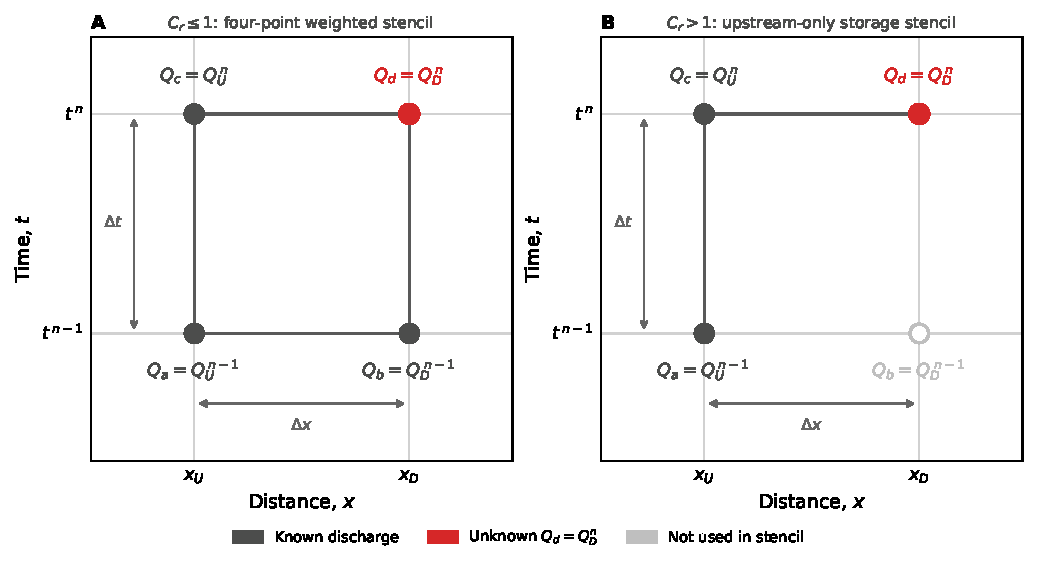
\includegraphics{./Figures/SFRKinematicWaveStencil.pdf}
	\caption[Space-time grid diagrams for the kinematic-wave finite-difference stencils used in the MODFLOW~6 SFR Package]{Space-time grid diagrams showing the nodal positions and variable names for the two kinematic-wave finite-difference stencils used in the MODFLOW~6 SFR Package ($Q_a = Q_U^{n-1}$, $Q_b = Q_D^{n-1}$, $Q_c = Q_U^n$, $Q_d = Q_D^n$). Filled nodes are known values; the red node ($Q_d$) is the unknown. \textit{A}, When $C_r \le 1$, all four nodes participate in the spatial and temporal difference approximations; \textit{B}, when $C_r > 1$, only the upstream temporal difference is retained for the storage term (the $Q_b$ node is not used)}
	\label{fig:sfr-stencil}
	\end{center}
\end{figure}

In the Preissmann scheme, the spatial derivative $\partial Q / \partial x$ is approximated at the temporal mid-point of the stencil as a weighted average of the spatial gradients at the two time levels, and the temporal derivative $\partial A / \partial t$ is approximated at the spatial mid-point as the average of the area changes at the two end nodes. Two discretizations arise depending on whether the Courant number is above or below unity.

When $C_r \le 1$, the scheme applies a temporal weighting parameter $\theta$ ($0.5 \le \theta \le 1$) to the spatial gradient term and averages the storage change over both time levels

\begin{equation}
	\label{eqn:sfr-residual-low-cr}
	\frac{\theta \left( Q_D^n - Q_U^n \right) + \left(1 - \theta \right) \left( Q_D^{n-1} - Q_U^{n-1} \right)}{\Delta x}
	+ \frac{1}{2} \frac{\left( A_D^n - A_D^{n-1} \right) + \left( A_U^n - A_U^{n-1} \right)}{\Delta t} = q_L ,
\end{equation}

\noindent where $q_L$ is the net lateral inflow per unit length at the current time step ($L^2 T^{-1}$), including contributions from overland runoff, evaporation, precipitation, groundwater exchange, and water mover fluxes. When $\theta = 1$, the scheme reduces to a fully implicit, first-order accurate spatial discretization. When $\theta = 0.5$, the scheme is second-order accurate in time and is equivalent to the Crank-Nicolson approximation.

When $C_r > 1$, the scheme uses only the current time step values at the upstream node for the storage term, which prevents the introduction of numerical instabilities that can arise when the wave speed exceeds the Courant stability limit for the $C_r \le 1$ scheme

\begin{equation}
	\label{eqn:sfr-residual-high-cr}
	\frac{Q_D^n - Q_U^n}{\Delta x} + \frac{A_U^n - A_U^{n-1}}{\Delta t} = q_L .
\end{equation}

\noindent Under this condition, the kinematic wave crest has already propagated through the entire reach within a single time step. Because the previous-time-level downstream state ($Q_D^{n-1}$, $A_D^{n-1}$) carries no information about the current wave front, it is excluded from the difference approximations; only the upstream area change $A_U^n - A_U^{n-1}$ captures the wave's passage through the reach.

The two cases may be written as a single residual function $f(Q_D^n)$

\begin{equation}
	\label{eqn:sfr-residual}
	f \left( Q_D^n \right) = \frac{\partial Q}{\partial x}\bigg|_\mathrm{fd} + \frac{\partial A}{\partial t}\bigg|_\mathrm{fd} - q_L = 0 ,
\end{equation}

\noindent where the finite-difference approximations correspond to equations~\ref{eqn:sfr-residual-low-cr} or \ref{eqn:sfr-residual-high-cr} depending on the Courant number. The unknown $Q_D^n$ enters through both the discharge term and the area term (because $A_D^n$ is determined from $Q_D^n$ via Manning's equation). Equation~\ref{eqn:sfr-residual} is solved iteratively using a Newton-Raphson method

\begin{equation}
	\label{eqn:sfr-newton}
	Q_D^{n, k+1} = Q_D^{n, k} - \frac{f \left( Q_D^{n, k} \right)}{f' \left( Q_D^{n, k} \right)} ,
\end{equation}

\noindent where the superscript $k$ denotes the Newton-Raphson iteration index and $f'$ is the derivative of the residual with respect to $Q_D^n$, approximated numerically.

\subsection{Reach Storage Change}

The change in water stored within a reach during a time step is required to ensure conservation of mass in the water budget. The storage change $\Delta S$ ($L^3 T^{-1}$) is calculated from the cross-sectional area values at the upstream and downstream ends of the reach at both time levels. For $C_r \le 1$

\begin{equation}
	\label{eqn:sfr-storage-low-cr}
	\Delta S = \frac{1}{2} \left[ \left( A_U^n + A_D^n \right) - \left( A_U^{n-1} + A_D^{n-1} \right) \right] \frac{\Delta x}{\Delta t} ,
\end{equation}

\noindent and for $C_r > 1$

\begin{equation}
	\label{eqn:sfr-storage-high-cr}
	\Delta S = \left( A_U^{n-1} - A_U^n \right) \frac{\Delta x}{\Delta t} .
\end{equation}

\noindent For $C_r \le 1$, the storage change is estimated from the trapezoidal average of the areas at both ends of the reach at both time levels. For $C_r > 1$, only the upstream area change is used, consistent with the assumption that the wave has already propagated through the reach. Note that the area differences in equations~\ref{eqn:sfr-storage-low-cr} and \ref{eqn:sfr-storage-high-cr} are the same terms that appear in the finite-difference residual (eqs.~\ref{eqn:sfr-residual-low-cr} and \ref{eqn:sfr-residual-high-cr}); the residual enforces continuity during the Newton-Raphson solve, while $\Delta S$ is computed separately once convergence is reached for use in the reach water budget. The appropriate expression is selected automatically based on the Courant number evaluated at each reach and time step. Equation~\ref{eqn:sfr-mf6-storage} provides the equivalent form as implemented in \mf, evaluated using the converged areas after Newton-Raphson convergence.

\subsection{Implementation in \mf}

The kinematic wave routing option is activated by specifying the \texttt{STORAGE} keyword in the OPTIONS block of the SFR Package input file \citep{modflow6gwf}. When \texttt{STORAGE} is activated, the SFR Package allocates storage for the upstream and downstream flow values from the previous time step and solves equation~\ref{eqn:sfr-residual} at each reach and time step using a Picard outer loop that also couples stream-aquifer exchange. The Picard loop iterates until the change in average reach depth (mean of upstream and downstream depths) falls below the \texttt{MAXIMUM\_DEPTH\_CHANGE} parameter (default $1 \times 10^{-5}$~m); for reaches with no groundwater exchange, the coupling is one-way and the loop reduces to a single iteration. The \texttt{MAXIMUM\_DEPTH\_CHANGE} parameter is package-wide and also controls the convergence tolerance for the standard instantaneous-flow formulation during steady-state stress periods. The kinematic wave routing option in \mf was validated against the modified Pinder-Sauer problem \citep{pinder1971numerical, lal2001modification}, which describes flood-wave attenuation due to bank storage effects and provides an analytical solution for stream-aquifer interaction under transient conditions.

\subsubsection{Lateral Source Term}

The net lateral source per unit length, $q_L$ ($L^2 T^{-1}$), combines all per-reach inflow and loss terms

\begin{equation}
	\label{eqn:sfr-qlat}
	q_L = \frac{q_r + q_{ro} - q_e}{\Delta x} - \frac{q_{gwf}}{\Delta x} ,
\end{equation}

\noindent where $q_r$ is direct precipitation onto the reach ($L^3 T^{-1}$), $q_{ro}$ is overland runoff into the reach ($L^3 T^{-1}$), $q_e$ is evaporation from the reach ($L^3 T^{-1}$), and $q_{gwf}$ is the groundwater exchange flux ($L^3 T^{-1}$, positive out of the stream). Dividing by $\Delta x$ converts these volumetric fluxes to the per-unit-length form required by equation~\ref{eqn:sfr-continuity}. All terms are evaluated at the current Picard iteration.

\subsubsection{Temporal Weighting}

The temporal weighting parameter $\theta$ defaults to 1.0 (fully implicit) and may be adjusted using the developer option \texttt{DEV\_STORAGE\_WEIGHT}. Values of $\theta$ between 0.5 and 1.0 are accepted; values less than 0.5 are not permitted because they can produce unstable solutions. A value of $\theta = 1.0$ provides maximum numerical stability at the cost of first-order temporal accuracy and is strongly recommended for all practical applications. When $\theta = 0.5$, equation~\ref{eqn:sfr-mf6-residual} becomes the Crank-Nicolson scheme \citep{CrankNicolson1947}, which is second-order accurate in time but may exhibit oscillations when $C_r < 1$ and the spatial discretization is coarse. The Courant number is evaluated at each reach and time step using the celerity estimated from the effective upstream inflow---the upstream discharge $Q_U^n$ adjusted for lateral contributions and groundwater exchange (eq.~\ref{eqn:sfr-courant}).

\subsubsection{Residual Function}

The finite-difference residual for each reach is evaluated at each Newton-Raphson iteration $k$ as

\begin{equation}
	\label{eqn:sfr-mf6-residual}
	f\!\left(Q_D^{n,k}\right) =
	\begin{dcases}
		\begin{aligned}
			&\dfrac{\theta \left(Q_D^{n,k} - Q_U^n\right) + \left(1-\theta\right)\!\left(Q_D^{n-1} - Q_U^{n-1}\right)}{\Delta x} \\[4pt]
			&\quad + \dfrac{\left(A_D^{n,k} - A_D^{n-1}\right) + \left(A_U^n - A_U^{n-1}\right)}{2\,\Delta t} - q_L
		\end{aligned}
		& C_r \le 1 \\[12pt]
		\dfrac{Q_D^{n,k} - Q_U^n}{\Delta x}
		+ \dfrac{A_U^n - A_U^{n-1}}{\Delta t} - q_L
		& C_r > 1
	\end{dcases} ,
\end{equation}

\noindent where $A_D^{n,k}$ is the wet cross-sectional area at the downstream end corresponding to $Q_D^{n,k}$, evaluated by inverting Manning's equation (eq.~\ref{eqn:sfr-manning}).

\subsubsection{Newton-Raphson Update}

Because the area $A_D^{n,k}$ depends nonlinearly on $Q_D^{n,k}$, equation~\ref{eqn:sfr-mf6-residual} is nonlinear and is solved with Newton-Raphson iteration, starting from the initial guess $Q_D^{n,0} = Q_D^{n-1}$ (the downstream discharge from the previous time step); when $Q_D^{n-1} = 0$---for example, at the start of a transient simulation or after a reach has gone dry---the initial guess is taken as $\tfrac{1}{2}(Q_U^n + Q_U^{n-1})$ instead. The derivative $f'$ is approximated by a forward finite difference using a small discharge perturbation $\delta$

\begin{equation}
	\label{eqn:sfr-mf6-deriv}
	f'\!\left(Q_D^{n,k}\right) \approx \frac{f\!\left(Q_D^{n,k} + \delta\right) - f\!\left(Q_D^{n,k}\right)}{\delta} ,
\end{equation}

\noindent and the discharge is updated as

\begin{equation}
	\label{eqn:sfr-mf6-update}
	Q_D^{n,k+1} = Q_D^{n,k} - \frac{f\!\left(Q_D^{n,k}\right)}{f'\!\left(Q_D^{n,k}\right)} .
\end{equation}

\noindent The updated discharge is floored at $10^{-30}$~m$^3$\,s$^{-1}$ to maintain a positive definite flow. Iteration continues until both the discharge correction and the residual fall below twice the perturbation $\delta$, or until the maximum of 100 Newton-Raphson iterations is reached

\begin{equation}
	\label{eqn:sfr-mf6-converge}
	\left| Q_D^{n,k+1} - Q_D^{n,k} \right| < 2\delta
	\quad \text{and} \quad
	\left| f\!\left(Q_D^{n,k+1}\right) \right| < 2\delta .
\end{equation}

\noindent The perturbation $\delta$ is set to $0.999 \times \texttt{MAXIMUM\_DEPTH\_CHANGE}$ and is used for the numerical celerity estimate (eq.~\ref{eqn:sfr-celerity-num}), the numerical derivative (eq.~\ref{eqn:sfr-mf6-deriv}), and the Newton-Raphson convergence test. The Picard depth-change tolerance equals \texttt{MAXIMUM\_DEPTH\_CHANGE} directly. Both are governed by the same input parameter.

\subsubsection{Reach Storage Change}

After Newton-Raphson convergence, the volumetric storage change $\Delta S$ ($L^3 T^{-1}$) for the reach water budget is computed from equations~\ref{eqn:sfr-storage-low-cr} and \ref{eqn:sfr-storage-high-cr} using the converged areas

\begin{equation}
	\label{eqn:sfr-mf6-storage}
	\Delta S =
	\begin{dcases}
		\dfrac{1}{2}\left[\left(A_U^n + A_D^n\right) - \left(A_U^{n-1} + A_D^{n-1}\right)\right] \dfrac{\Delta x}{\Delta t}
		& C_r \le 1 \\[10pt]
		\left(A_U^{n-1} - A_U^n\right) \dfrac{\Delta x}{\Delta t}
		& C_r > 1
	\end{dcases} .
\end{equation}

\subsection{Example: Effect of Courant Number on Downstream Hydrograph}

The accuracy of the \mf finite-difference scheme (eq.~\ref{eqn:sfr-mf6-residual}) is illustrated by comparing the computed downstream hydrograph against the exact kinematic-wave solution for a single rectangular reach with a sinusoidal upstream boundary condition.

\subsubsection{Problem Setup}

The test reach has length $\Delta x = 500$ m, width $B = 10$ m, bed slope $S_0 = 0.001$, and Manning's roughness $n = 0.03$ s$\,$m$^{-1/3}$. No lateral inflow is applied ($q_L = 0$). The upstream boundary hydrograph is

\begin{equation}
	\label{eqn:sfr-example-qin}
	Q_U(t) = Q_0 \left[ 1 + 0.4 \sin\!\left( \frac{2\pi t}{T_\mathrm{wave}} \right) \right] ,
\end{equation}

\noindent where the base flow is $Q_0 = 5$ m$^3$s$^{-1}$ and the wave period is $T_\mathrm{wave} = 10\,T$. The wave celerity at base flow is $c_0 \approx 1.18$ m$\,$s$^{-1}$, giving a travel time of $T = \Delta x / c_0 \approx 423$ s.

\subsubsection{Exact Solution}

For the linearized kinematic wave with constant celerity and no lateral inflow, the governing equation~\ref{eqn:sfr-continuity} reduces to the pure advection equation

\begin{equation}
	\label{eqn:sfr-example-advection}
	\frac{\partial Q}{\partial t} + c_0 \frac{\partial Q}{\partial x} = 0 ,
\end{equation}

\noindent whose exact solution is a pure translation: the downstream hydrograph equals the upstream hydrograph delayed by the travel time $T$

\begin{equation}
	\label{eqn:sfr-example-exact}
	Q_D^\mathrm{exact}(t) = Q_U(t - T) .
\end{equation}

\subsubsection{Finite-Difference Results}

The \mf scheme is run at six Courant numbers (0.5, 0.75, 1.0, 1.25, 1.5, and 2.0) obtained by varying the time step $\Delta t = C_r \, T$. The temporal weighting parameter is held at the default value $\theta = 1.0$. Results are compared against the exact solution (eq.~\ref{eqn:sfr-example-exact}) in figure~\ref{fig:sfr-kinwave}. For $C_r \le 1$ (fig.~\ref{fig:sfr-kinwave}\textit{A}), the scheme applies the four-point weighted stencil (eq.~\ref{eqn:sfr-residual-low-cr}). The $C_r = 1$ solution is nearly exact, recovering the pure translation with negligible diffusion. As $C_r$ decreases below 1, increasing numerical diffusion smooths the peaks and troughs of the downstream hydrograph. For $C_r > 1$ (fig.~\ref{fig:sfr-kinwave}\textit{B}), the scheme switches to the upstream-only storage stencil (eq.~\ref{eqn:sfr-residual-high-cr}). At $C_r = 1.25$ the downstream hydrograph is well-recovered, but at higher Courant numbers the larger time steps undersample the wave period, producing progressively greater phase and amplitude errors. These results confirm that Courant numbers near unity provide the best balance between computational efficiency and accuracy for the kinematic wave option.

\begin{figure}[!ht]
	\begin{center}
	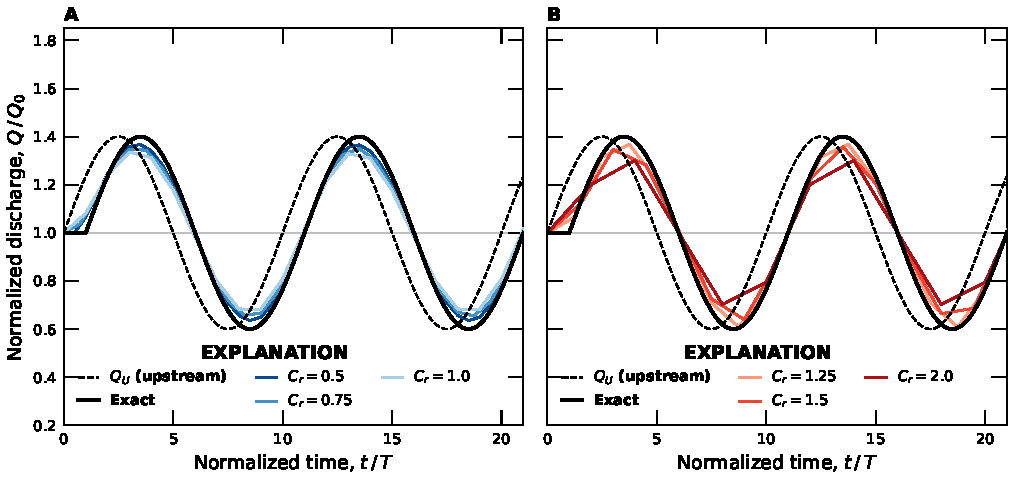
\includegraphics{./Figures/SFRKinematicWave.pdf}
	\caption[Graphs comparing the MODFLOW~6 kinematic-wave scheme against the exact solution at six Courant numbers for a single rectangular reach]{Graphs comparing the MODFLOW~6 kinematic-wave finite-difference scheme against the exact kinematic-wave solution for a single rectangular reach ($\Delta x = 500$ m, $B = 10$ m, $S_0 = 0.001$, $n = 0.03$ s$\,$m$^{-1/3}$) with a sinusoidal upstream boundary condition (eq.~\ref{eqn:sfr-example-qin}) and no lateral inflow. The base flow is $Q_0 = 5$ m$^3$s$^{-1}$, the temporal weighting parameter is $\theta = 1.0$, and time is normalized by the kinematic-wave travel time $T = \Delta x / c_0 \approx 423$ s. \textit{A}, Courant numbers $C_r \le 1$ (0.5, 0.75, and 1.0) showing increasing numerical diffusion as $C_r$ decreases from unity; \textit{B}, Courant numbers $C_r > 1$ (1.25, 1.5, and 2.0) showing increasing phase and amplitude errors as the time step coarsens}
	\label{fig:sfr-kinwave}
	\end{center}
\end{figure}

\subsection{Practical Guidance}

\subsubsection{Choosing a Suitable Time Step}

The accuracy of the kinematic-wave scheme depends on the Courant number $C_r = c\,\Delta t / \Delta x$ (eq.~\ref{eqn:sfr-courant}), and figure~\ref{fig:sfr-kinwave} demonstrates that $C_r$ near unity provides the best balance between accuracy and computational efficiency. A practical starting point is therefore to target $C_r \approx 1$ at or near the expected base flow.

For a rectangular channel, the kinematic wave celerity can be estimated from Manning's equation. When the channel is hydraulically wide (width $B$ much larger than flow depth $d$), the hydraulic radius $R \approx d$, and the celerity simplifies to approximately five thirds of the mean flow velocity $\bar{V} = Q / A$

\begin{equation}
	\label{eqn:sfr-celerity-wide}
	c \approx \frac{5}{3} \bar{V} .
\end{equation}

\noindent Setting $C_r = 1$ and solving for the time step gives the optimal value

\begin{equation}
	\label{eqn:sfr-dt-opt}
	\Delta t_\mathrm{opt} = \frac{\Delta x}{c} \approx \frac{3\,\Delta x\,A_0}{5\,Q_0} ,
\end{equation}

\noindent where $A_0$ and $Q_0$ are the cross-sectional area and discharge at base flow. The optimal time step scales linearly with reach length, so doubling $\Delta x$ doubles $\Delta t_\mathrm{opt}$. Because wave celerity increases with discharge for Manning's-equation channels (equation~\ref{eqn:sfr-celerity-wide}), the Courant number during high-flow conditions will exceed the base-flow value; the code accommodates this automatically by switching to the upstream-only storage stencil (eq.~\ref{eqn:sfr-residual-high-cr}) when $C_r > 1$.

Figure~\ref{fig:sfr-courant} provides two complementary views of the Courant number for a representative rectangular channel ($B = 10$ m, $n = 0.035$). Panel~\textit{A} shows the Courant number $C_r = c\,\Delta t / \Delta x$ evaluated at a reference time step of 10 minutes and reach length of 500 m; for other choices, $C_r$ scales proportionally with $\Delta t$ and inversely with $\Delta x$. The gray band marks the recommended range $0.5 \le C_r \le 2$. As discharge or bed slope increases, the wave celerity rises and the Courant number increases for a fixed time step; steeper and higher-flow reaches require shorter time steps to stay within the acceptable range. Panel~\textit{B} shows the optimal time step $\Delta t_\mathrm{opt} = \Delta x / c$ (minutes) required to achieve $C_r = 1$ for a 500-m reach. The dashed horizontal lines mark common model time steps of 5, 15, and 60 minutes; where a slope curve lies above a reference line, the corresponding time step gives $C_r < 1$ (tends toward excessive diffusion), and where it lies below, the time step gives $C_r > 1$ (tends toward undersampling). The acceptable range spans approximately half to twice the curve value, corresponding to $0.5 \le C_r \le 2$.

When a model contains reaches with different slopes and geometries, the time step should satisfy $C_r \approx 1$ for the reach with the largest celerity-to-length ratio $c / \Delta x$, because all reaches share the same global time step. Courant numbers between approximately 0.5 and 2 are generally acceptable across the network; values outside this range will introduce progressively greater numerical diffusion or phase error (fig.~\ref{fig:sfr-kinwave}).

Because the code does not write celerity or Courant numbers to any model output file, Courant numbers must be estimated manually before selecting a time step. Equations~\ref{eqn:sfr-celerity-wide} and \ref{eqn:sfr-courant} provide a convenient starting point; figure~\ref{fig:sfr-courant} shows pre-computed values for a range of discharges and bed slopes. Confirming that $C_r$ lies within the acceptable range at expected base-flow conditions---and not only at mean flow---is recommended before committing to a time step for a full simulation.

\begin{figure}[!ht]
	\begin{center}
	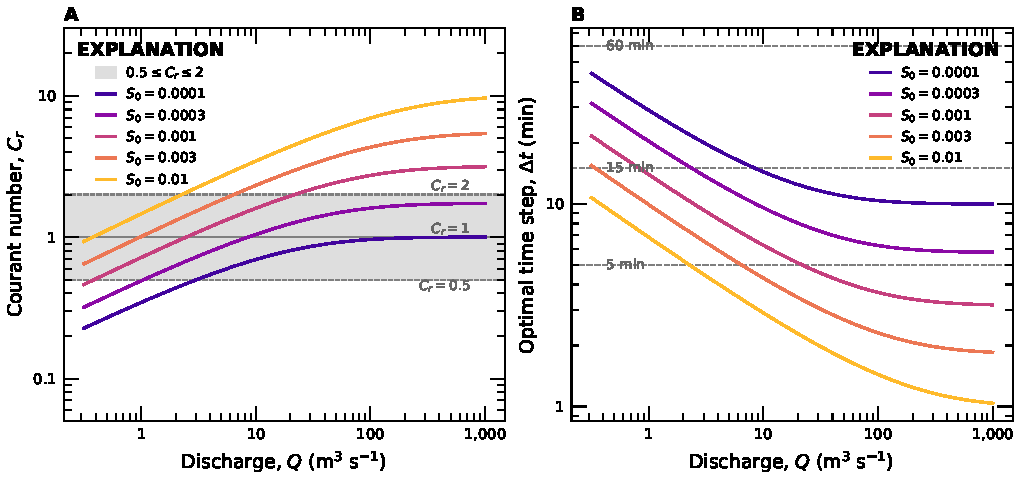
\includegraphics{./Figures/SFRKinematicWaveCourant.pdf}
	\caption[Graphs showing kinematic-wave Courant number and optimal time step as functions of discharge and bed slope]{Graphs showing kinematic-wave routing guidance for a rectangular channel ($B = 10$ m, $n = 0.035$) and reach length of 500 m, as functions of discharge for five bed slopes. Both axes are logarithmic. \textit{A}, Courant number $C_r = c\,\Delta t / \Delta x$ for a reference time step of 10 minutes; $C_r$ scales as $(\Delta t / 10 \text{ min}) \times (500 \text{ m} / \Delta x)$ for other choices. The gray band marks the recommended range $0.5 \le C_r \le 2$; \textit{B}, Optimal time step $\Delta t_\mathrm{opt} = \Delta x / c$ (minutes) for $C_r = 1$. Dashed horizontal lines show common model time steps; where a slope curve lies above a line, that time step gives $C_r < 1$, and where it lies below, $C_r > 1$. The acceptable range is approximately half to twice the curve value}
	\label{fig:sfr-courant}
	\end{center}
\end{figure}

\subsubsection{Applicability Conditions}

The kinematic wave approximation is most appropriate for steep to moderately sloped, free-draining channels where backwater and inertial effects are negligible. A widely used criterion for assessing applicability is the dimensionless kinematic wave number \citep{WoolhiserLiggett1967, PonceLiSimons1978}

\begin{equation}
	\label{eqn:sfr-kw-param}
	K = \frac{S_0 \, \Delta x}{F_0^2 \, d_0} ,
\end{equation}

\noindent where $d_0$ is the base-flow depth and $F_0 = \bar{V}_0 / \sqrt{g\,d_0}$ is the Froude number at base flow. Values of $K \gtrsim 10$ indicate that the kinematic wave is a good approximation; values of $K < 5$ suggest that momentum storage, pressure gradients, or backwater effects are important and that the kinematic wave may produce significant errors \citep{Ponce1991}. The kinematic wave option should not be used in the following situations:

\begin{itemize}

	\item \textit{Very mild slopes} ($S_0 \lesssim 10^{-4}$). Longitudinal pressure gradients and downstream backwater effects become important relative to friction, and the diffusive wave or full dynamic wave is more appropriate.

	\item \textit{Regulated or ponded reaches}. Reaches immediately downstream of dams, weirs, or tidal boundaries are subject to imposed water-surface profiles that invalidate the kinematic assumption.

	\item \textit{Reaches with strong stream-aquifer exchange}. Where large and rapidly varying groundwater seepage substantially alters the flow depth within a reach, the simple celerity estimate may be unreliable and convergence may be slow.

	\item \textit{Supercritical or near-critical flow} ($F_0 \ge 1$). The kinematic wave approximation assumes subcritical flow; reaches with very steep slopes and high velocities may reach or exceed critical conditions at high discharges.

\end{itemize}

\subsubsection{Potential Numerical Problems}

Several numerical issues can arise when using the kinematic-wave option:

\begin{itemize}

	\item \textit{Artificial smoothing of flood peaks} ($C_r \ll 1$). When the time step is much shorter than $\Delta t_\mathrm{opt}$, the numerical scheme introduces an artificial spreading effect---called numerical diffusion---that is not present in the physical system. The result is that computed peak flows at the downstream end of a reach are lower than they should be, and the flood hydrograph appears broader and more rounded: the rising limb rises more gradually, the peak is reduced, and the recession drains more slowly. The wave still translates at roughly the correct speed, but its shape is progressively damped with each time step. Figure~\ref{fig:sfr-kinwave}\textit{A} illustrates this for $C_r = 0.5$ and $C_r = 0.75$: both solutions show the correct timing but underestimate the peak and overestimate the through relative to the exact solution. Increasing the time step, or subdividing long reaches into shorter segments to reduce $\Delta x$, brings $C_r$ closer to unity and reduces the smoothing.

	\item \textit{Flood-wave timing and peak-flow errors} ($C_r \gg 1$). When the time step is much larger than $\Delta t_\mathrm{opt}$, the scheme takes too few samples of the upstream hydrograph to reconstruct its shape accurately. The practical consequence is that the computed downstream hydrograph can show the flood peak arriving at the wrong time and at the wrong magnitude---peak flows are underestimated and the through between successive waves is filled in, making the hydrograph appear flatter and more spread out than the true response. The effect worsens as $C_r$ increases beyond 2. Figure~\ref{fig:sfr-kinwave}\textit{B} illustrates this for $C_r = 1.5$ and $C_r = 2$: both solutions preserve the general shape but drift progressively in phase and underestimate the peak. Reducing the time step so that $C_r \lesssim 2$ is recommended; for applications where accurate flood timing or peak-flow magnitude is important, targeting $C_r$ close to 1 is preferable.

	\item \textit{Oscillatory solutions} ($\theta < 1$). Reducing the temporal weighting parameter below 1 using the developer option \texttt{DEV\_STORAGE\_WEIGHT} can cause oscillatory solutions at low Courant numbers because the Crank-Nicolson scheme is prone to dispersion errors near $C_r = 0$. The default value $\theta = 1.0$ is strongly recommended for all practical applications.

	\item \textit{Convergence failures on steep wave fronts}. Hydrographs with a very rapid rise---for example, from a sudden change in an upstream boundary condition---can create steep wave fronts that challenge the Newton-Raphson solver (eq.~\ref{eqn:sfr-mf6-update}). Reducing the time step so that the front is better resolved usually resolves the problem.

	\item \textit{Slow convergence with strong groundwater exchange}. The kinematic-wave residual is evaluated within the outer Picard loop that couples stream-aquifer exchange. Reaches with large or rapidly varying leakage fluxes may require more outer iterations to converge. If the model fails to converge within the allowed number of outer iterations, increasing \texttt{OUTER\_MAXIMUM} in the IMS NONLINEAR block or reducing the time step may help.

	\item \textit{Mass-balance drift from discharge flooring}. When the Newton-Raphson update would produce a negligible or negative discharge, the downstream flow is floored at $10^{-30}$~m$^3$\,s$^{-1}$. In reaches that intermittently go dry, repeated flooring can introduce small mass-balance errors. Monitoring the SFR volumetric budget---particularly the storage term---at each time step is recommended to verify that cumulative errors remain small.

\end{itemize}

\subsubsection{Interaction with the SFR Package}

The \texttt{STORAGE} keyword activates kinematic-wave routing for all reaches in the SFR Package for the duration of a simulation. The option applies only during transient stress periods; steady-state stress periods, including those used to establish initial conditions before a transient simulation, use the standard instantaneous-flow SFR formulation regardless of whether \texttt{STORAGE} is specified, so mixed steady-state and transient simulations are handled automatically.

Because individual reaches in a network can differ markedly in length and slope, the Courant number will vary from reach to reach for a given time step. A preliminary run using a short time step---for example, one tenth of the estimated $\Delta t_\mathrm{opt}$ for the fastest reach---can help identify which reaches have problematic Courant numbers. Once the celerity field is understood, the time step can be increased to the largest value that keeps $C_r$ within the acceptable range for the most sensitive reaches. Subdividing unusually long reaches into shorter segments, or merging very short adjacent reaches, can help to equalize Courant numbers across the network and allow a longer global time step.
